\begin{tframe}{Conclusion}
    \textbf{Agentic Graph \gls{rag}} was introduced to deliver contextual and explainable recommendations for research collaborators by combining \textbf{\glspl{kg}} and \textbf{\glspl{llm}}.
    
    \vspace{0.5em}
    \textbf{Evaluation Highlights:}
    \begin{itemize}
      \item High-quality and contextual reasoning, reduced hallucinations
      \item Areas needing improvement: \textit{consistency} and \textit{context retrieval}
    \end{itemize}
    
    %\vspace{0.5em}
    \begin{columns}
      \begin{column}{0.52\textwidth}
        \begin{itemize}
          {\scriptsize
          \item This thesis work has been submitted to the \textbf{Society 5.0 conference}%\footnote{\url{https://www.conference-society5.org}}
          \item A journal version is in preparation for submission to the \textbf{Semantic-Web Journal}%\footnote{\url{https://www.semantic-web-journal.net/blog/special-issue-large-language-models-generative-ai-and-knowledge-graphs}}
          }
        \end{itemize}

        %\vspace{0.2cm}

      \end{column}
      \begin{column}{0.4\textwidth}
        %\vspace{-.5cm}
        \begin{figure}[htbp]
          \centering
          \rotatebox{-5}{\fbox{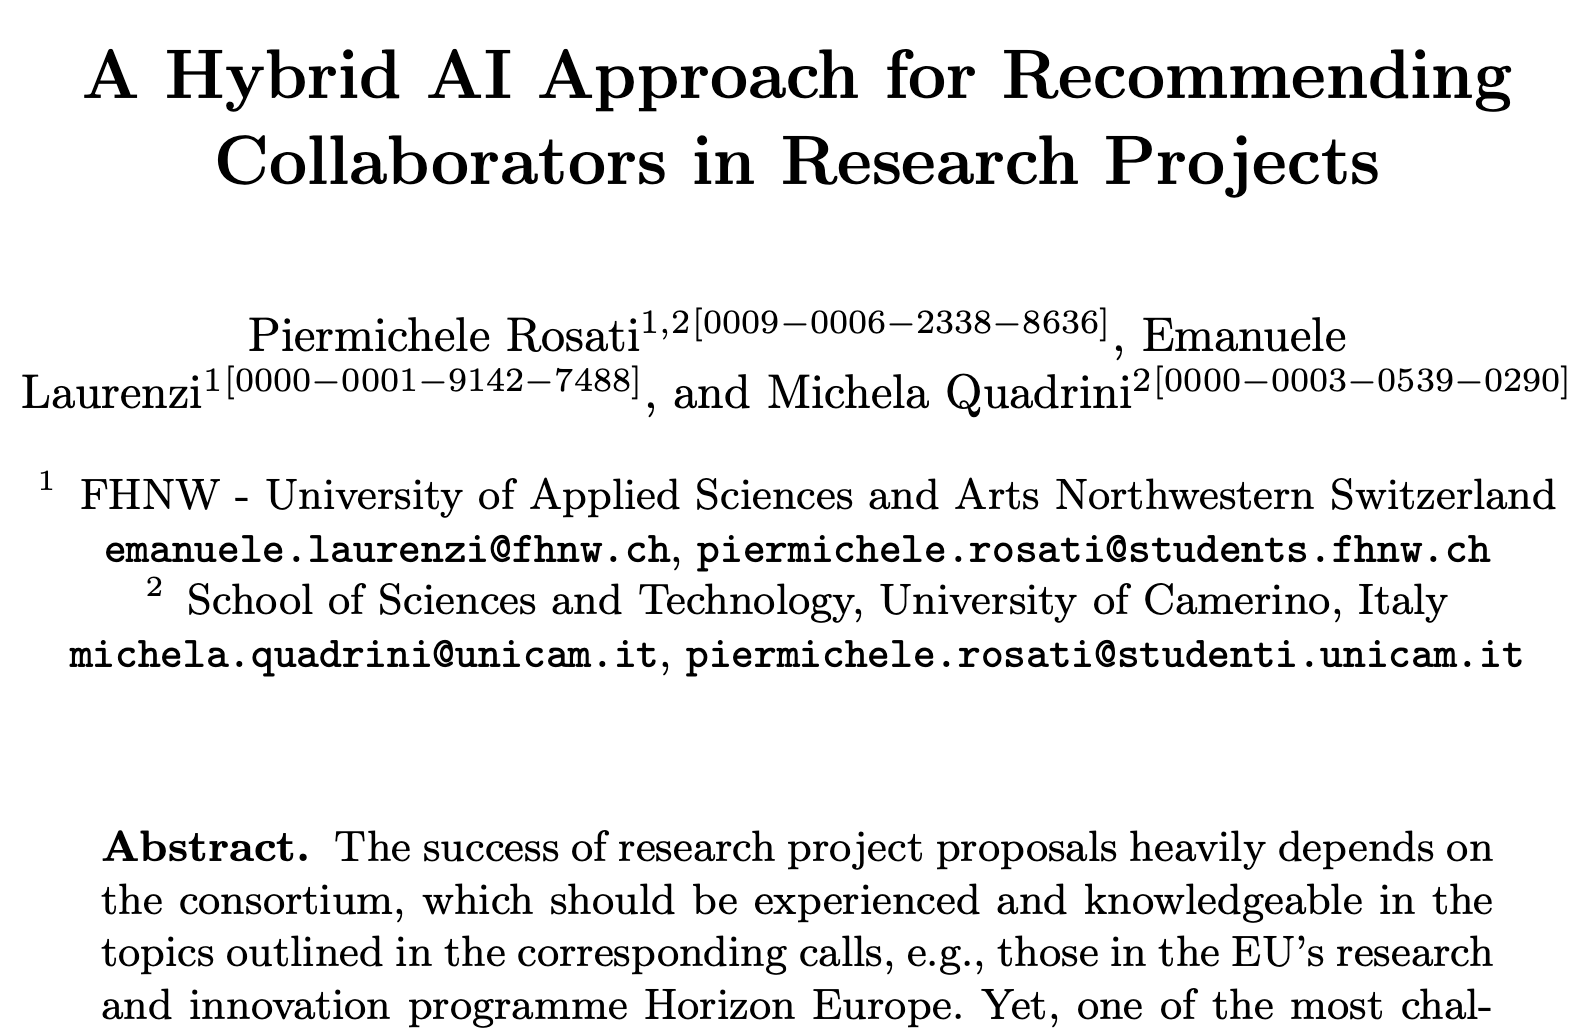
\includegraphics[width=.75\textwidth]{../img/conclusion/society-paper.png}}}
      \end{figure}
      \end{column}
  \end{columns}
\end{tframe}